\begin{figure}[H]
    \centering

    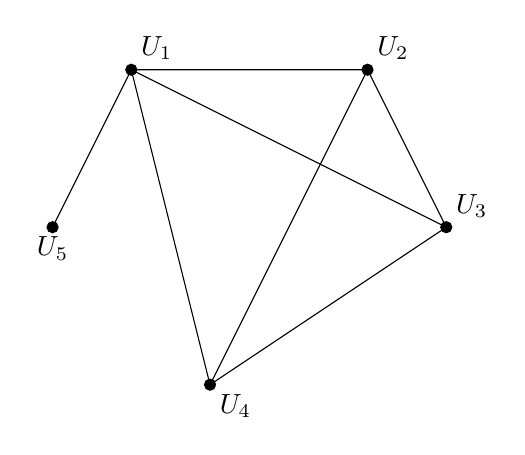
\begin{tikzpicture}
        
        % Points
        \draw[fill=black] (1,1) circle (2pt) node[below] {$U_5$};
        \draw[fill=black] (2,3) circle (2pt) node[above right] {$U_1$};
        \draw[fill=black] (5,3) circle (2pt) node[above right] {$U_2$};
        \draw[fill=black] (6,1) circle (2pt) node[above right] {$U_3$};
        \draw[fill=black] (3,-1) circle (2pt) node[below right] {$U_4$};

        
        % Lines
        \draw (1,1) -- (2,3) -- (5,3) -- (6,1) -- (3, -1) -- (2, 3);
        \draw (6,1) -- (2,3);
        \draw (3, -1) -- (5, 3);
    \end{tikzpicture}
    
\end{figure}